\documentclass[11pt]{beamer}
\usetheme{Boadilla}

\usepackage{tabu}
\usepackage[linesnumbered,ruled,vlined]{algorithm2e}
\usepackage{xcolor}
\usepackage{hyperref}

%\newcommand{\tabitem}{%
%  \usebeamertemplate{itemize item}\hspace*{\labelsep}}

\title{Ethereum Virtual Machine Bytecode Analyzer}
\subtitle{Guided Research}
\author{Alexander Roschlaub}
\date{\today}

\begin{document}

\begin{frame}
\titlepage
\end{frame}

\begin{frame}{Background}
\framesubtitle{Security Analysis Framework for Smart Contracts}
    \begin{enumerate}
        \item source code is not available (77\% of unique smart contracts\footnotemark)
        \item only visible at the level of bytecode (e.g. gas consumption)
        \item optimizations performed by the compiler 
    \end{enumerate}
    \footnotetext[1]{01.2018 - \href{https://www.usenix.org/system/files/conference/usenixsecurity18/sec18-zhou.pdf}{EthIR}}
\end{frame}

\begin{frame}
\frametitle{Outline}
\tableofcontents
\end{frame}


\section{Bytecode Transformation}

\begin{frame}{Bytecode Transformation(1): Vectorization}
Input (Bytecode): 6080604052348015600f57600080fd5b50600436106045
\onslide<2->
Output: Objectsvector
\begin{figure}
    \centering
    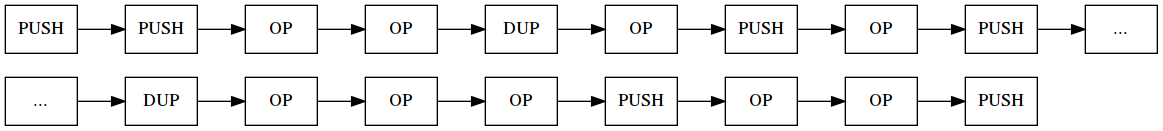
\includegraphics[scale=0.25]{figures/norm1_objects.png}
\end{figure}
\onslide<3->
Filtering of Push Bytes:
\begin{figure}
    \centering
    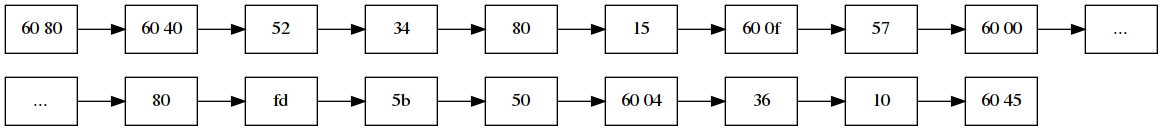
\includegraphics[scale=0.25]{figures/norm1.png}
\end{figure}
Implemented: Operation (base case), Push, Swap, Dup
\end{frame}

\begin{frame}{Definition: Basic Block}
\begin{columns}
\column{0.5\textwidth}
    \begin{itemize}
        \item $0 \ldots n$ predecessors
        \item content: $1 \ldots i$ operations
        \item $0 \ldots k$ successors (Jump, Fallthrough).
    \end{itemize}
\column{0.5\textwidth}
\begin{figure}
    \centering
    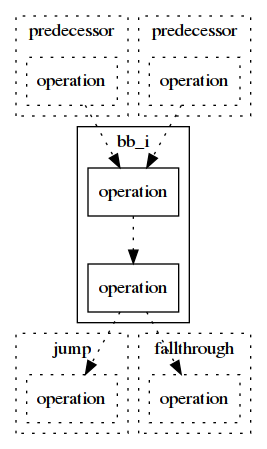
\includegraphics[scale=0.4]{figures/bb_def.png}
\end{figure}
\end{columns}
\end{frame}

\begin{frame}{Bytecode Transformation(2): Basic Block Grouping}
Input: Objectsvector
\begin{figure}
    \centering
    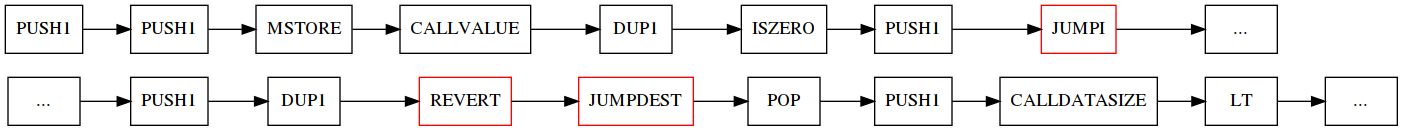
\includegraphics[scale=0.24]{figures/norm2_input.png}
\end{figure}
\onslide<2->
\begin{enumerate}
    \item Group into Basic Blocks
    \item Assign fallthrough successors
    \onslide<3->
    \item \textcolor{red}{Problem:} Position encoded jump destinations as stack items
\end{enumerate}
\onslide<2->
\begin{figure}
    \centering
    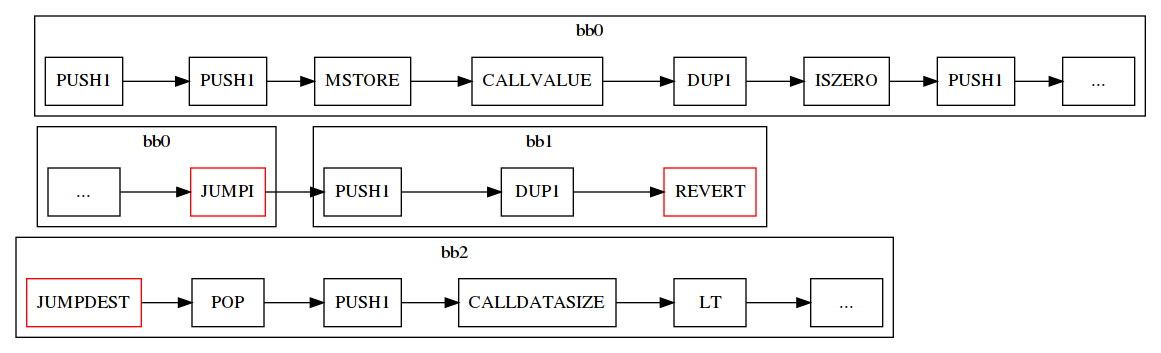
\includegraphics[scale=0.25]{figures/norm2_step.png}
    %\caption{Group into Basic Blocks with possible assignment of Fallthrough Successor}
\end{figure}
\end{frame}

\begin{frame}{Basic Block Grouping: Adjust Jump Pointer}
\begin{columns}
\column{0.3\textwidth}
\only<1>{
    \begin{figure}
        \centering
        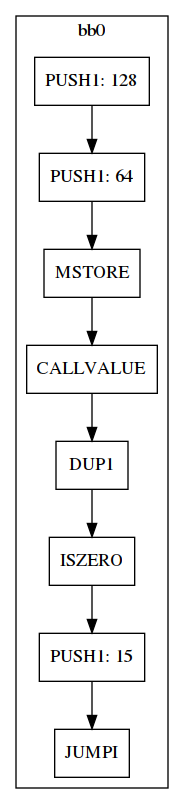
\includegraphics[scale=0.25]{figures/stack/cfg_stack0.png}
    \end{figure}
}
\only<2>{
    \begin{figure}
        \centering
        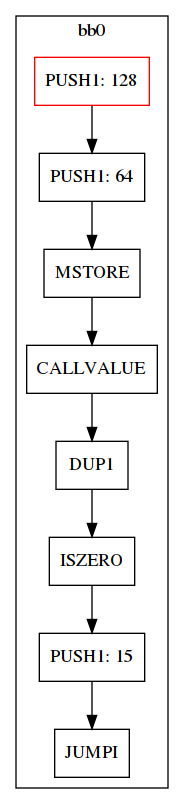
\includegraphics[scale=0.25]{figures/stack/cfg_stack1.png}
    \end{figure}
}
\only<3>{
    \begin{figure}
        \centering
        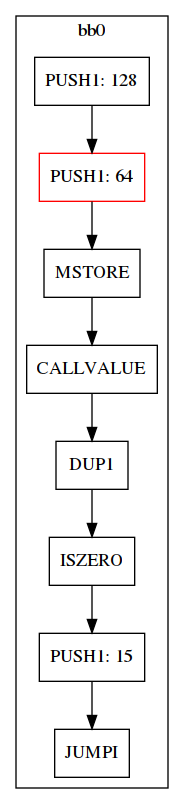
\includegraphics[scale=0.25]{figures/stack/cfg_stack2.png}
    \end{figure}
}
\only<4>{
    \begin{figure}
        \centering
        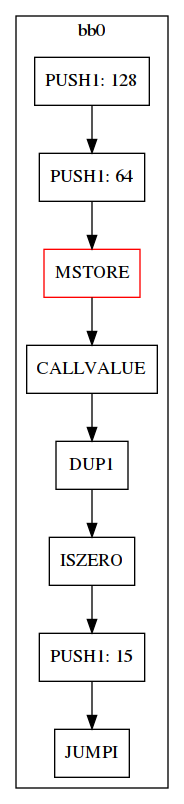
\includegraphics[scale=0.25]{figures/stack/cfg_stack3.png}
    \end{figure}
}
\only<5>{
    \begin{figure}
        \centering
        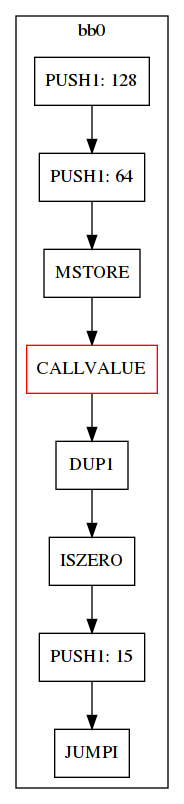
\includegraphics[scale=0.25]{figures/stack/cfg_stack4.png}
    \end{figure}
}
\only<6>{
    \begin{figure}
        \centering
        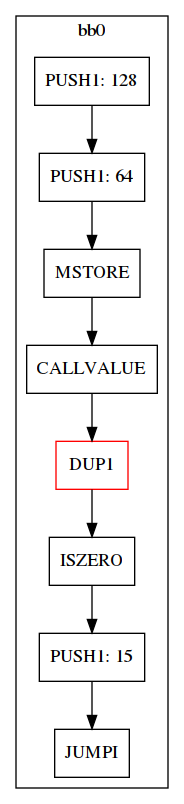
\includegraphics[scale=0.25]{figures/stack/cfg_stack5.png}
    \end{figure}
}
\only<7>{
    \begin{figure}
        \centering
        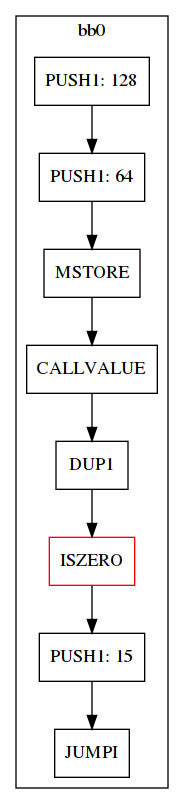
\includegraphics[scale=0.25]{figures/stack/cfg_stack6.png}
    \end{figure}
}
\only<8>{
    \begin{figure}
        \centering
        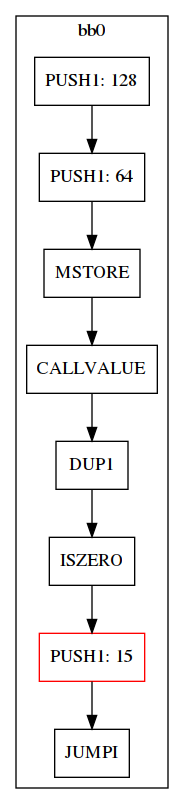
\includegraphics[scale=0.25]{figures/stack/cfg_stack7.png}
    \end{figure}
}
\only<9>{
    \begin{figure}
        \centering
        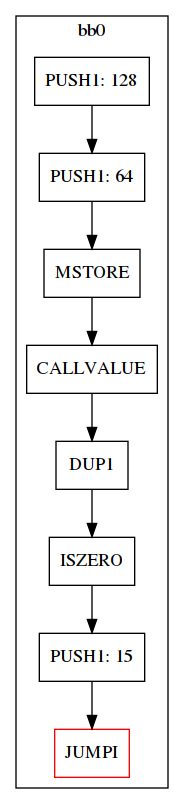
\includegraphics[scale=0.25]{figures/stack/cfg_stack8.png}
    \end{figure}
}
\column{0.7\textwidth}
\only<1>{
    Each Operation has defined parameters:
    \begin{itemize}
        \item $\alpha$: Number of elements pushed onto the stack
        \item $\delta$: Number of elements popped from the stack
        \item 0 as dummy element (256 bit)
    \end{itemize}
}
\only<2>{
\newline PUSH1:
\begin{itemize}
    \item $\alpha$: 1
    \item $\delta$: 0
\end{itemize}
    \begin{figure}
        \centering
        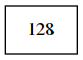
\includegraphics[scale=0.4]{figures/stack/stack1.png}
        \caption{Stack State After}
    \end{figure}
}
\only<3>{
    \begin{figure}
        \centering
        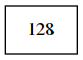
\includegraphics[scale=0.4]{figures/stack/stack1.png}
        \caption{Stack State Before}
    \end{figure}
    PUSH1:
    \begin{itemize}
          \item $\alpha$: 1
          \item $\delta$: 0
    \end{itemize}
    \begin{figure}
        \centering
        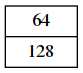
\includegraphics[scale=0.4]{figures/stack/stack2.png}
        \caption{Stack State After}
    \end{figure}
}
\only<4>{
    \begin{figure}
        \centering
        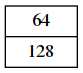
\includegraphics[scale=0.4]{figures/stack/stack2.png}
        \caption{Stack State Before}
    \end{figure}
    MSTORE:
    \begin{itemize}
        \item $\alpha$: 0
        \item $\delta$: 2
    \end{itemize}
    \begin{figure}
        \centering
        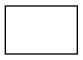
\includegraphics[scale=0.4]{figures/stack/stack3.png}
        \caption{Stack State After}
    \end{figure}
}
\only<5>{
    \begin{figure}
        \centering
        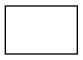
\includegraphics[scale=0.4]{figures/stack/stack3.png}
        \caption{Stack State Before}
    \end{figure}
    CALLVALUE:
    \begin{itemize}
        \item $\alpha$: 1
        \item $\delta$: 0
    \end{itemize}
    \begin{figure}
        \centering
        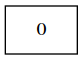
\includegraphics[scale=0.5]{figures/stack/stack4.png}
        \caption{Stack State After}
    \end{figure}
}
\only<6>{
    \begin{figure}
        \centering
        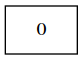
\includegraphics[scale=0.5]{figures/stack/stack4.png}
        \caption{Stack State Before}
    \end{figure}
    DUP1:
    \begin{itemize}
        \item $\alpha$: 1
        \item $\delta$: 1
    \end{itemize}
    \begin{figure}
        \centering
        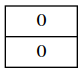
\includegraphics[scale=0.5]{figures/stack/stack5.png}
        \caption{Stack State After}
    \end{figure}
}
\only<7>{
    \begin{figure}
        \centering
        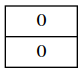
\includegraphics[scale=0.5]{figures/stack/stack5.png}
        \caption{Stack State Before}
    \end{figure}
    ISZERO:
    \begin{itemize}
        \item $\alpha$: 1
        \item $\delta$: 1
    \end{itemize}
    \begin{figure}
        \centering
        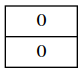
\includegraphics[scale=0.5]{figures/stack/stack6.png}
        \caption{Stack State After}
    \end{figure}
}
\only<8>{
    \begin{figure}
        \centering
        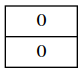
\includegraphics[scale=0.5]{figures/stack/stack6.png}
        \caption{Stack State Before}
    \end{figure}
    PUSH1:
    \begin{itemize}
        \item $\alpha$: 1
        \item $\delta$: 0
    \end{itemize}
    \begin{figure}
        \centering
        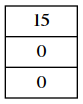
\includegraphics[scale=0.5]{figures/stack/stack7.png}
        \caption{Stack State After}
    \end{figure}
}
\only<9>{
    \begin{figure}
        \centering
        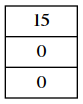
\includegraphics[scale=0.5]{figures/stack/stack7.png}
        \caption{Stack State Before}
    \end{figure}
    JUMPI:
    \begin{itemize}
        \item $\alpha$: 0
        \item $\delta$: 2
    \end{itemize}
    \begin{figure}
        \centering
        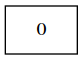
\includegraphics[scale=0.5]{figures/stack/stack8.png}
        \caption{Stack State After}
    \end{figure}
}
\end{columns}
\end{frame}

\begin{frame}{Basic Block Grouping: Merging Paths Problem}
\begin{columns}
\column{0.7\textwidth}
\begin{itemize}
    \item<1-> Problem: Only the fallthrough predecessor is known beforehand
    \item<2-> Condition: Evaluation of jump positions only
    \item<3-> Solution: Error output for duplicate assignments (Better: Fixpoint Iteration)
\end{itemize}
\column{0.3\textwidth}
    \begin{figure}
        \centering
        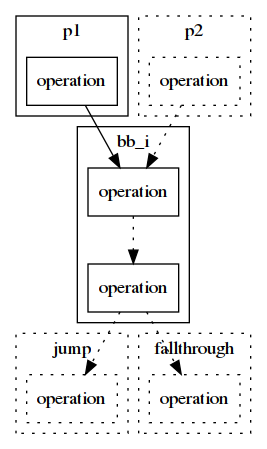
\includegraphics[scale=0.35]{figures/mpp1.png}
    \end{figure}
\end{columns}
\end{frame}

\section{Stack Abstraction}

\begin{frame}{CFG vs optimized CFG}
\begin{columns}
\column{0.3\textwidth}
\begin{figure}
    \centering
    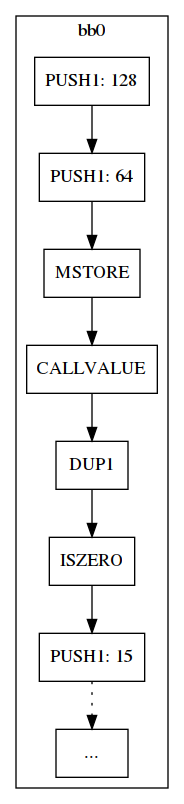
\includegraphics[scale=0.2]{figures/cfg_normal_1.png}
    \caption{CFG(I)}
\end{figure}
\column{0.3\textwidth}
\begin{figure}
    \centering
    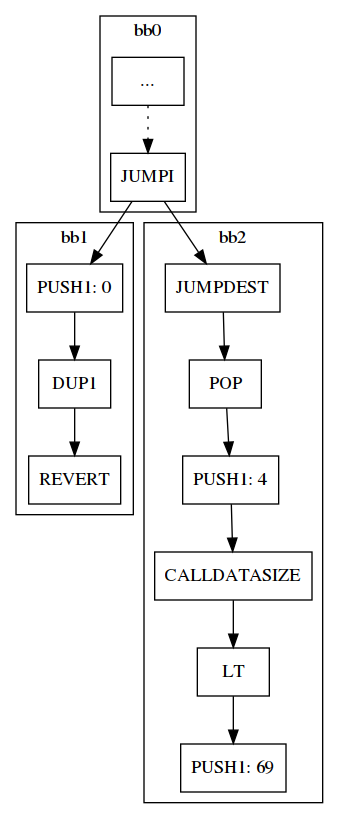
\includegraphics[scale=0.2]{figures/cfg_normal_2.png}
    \caption{CFG(II)}
\end{figure}
\onslide<2->
\column{0.3\textwidth}
\begin{figure}
    \centering
    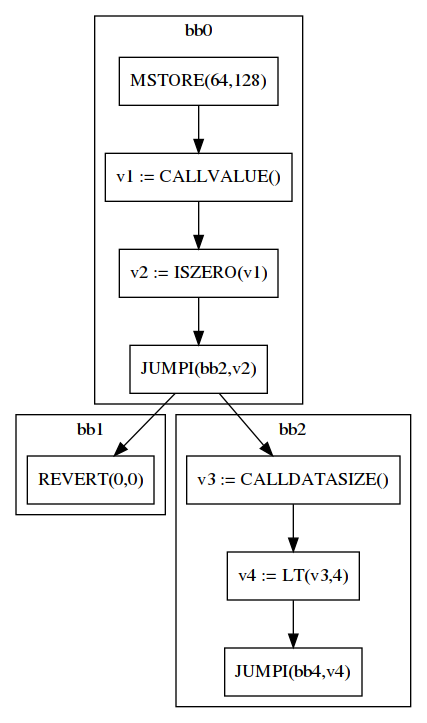
\includegraphics[scale=0.2]{figures/graph3.png}
    \caption{Optimized CFG}
\end{figure}
\end{columns}
\end{frame}

\begin{frame}{Stack Abstraction: First Idea}
\begin{columns}
\column{0.7\textwidth}
    \begin{enumerate}
        \item<1-4> Replicate the Basic Blocks from the CFG with empty content
        \item<2-4> Recursive instantiation of Basic Blocks
            \begin{enumerate}
                \item<3-4> Transform the Operations into Instructions
                \item<4> Pass the stack to successors
            \end{enumerate}
    \end{enumerate}
\column{0.3\textwidth}
\only<1>{
\begin{figure}
    \centering
    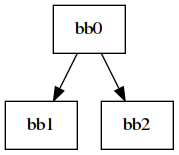
\includegraphics[scale=0.4]{figures/abstraction1.png}
\end{figure}
}
\only<2>{
\begin{figure}
    \centering
    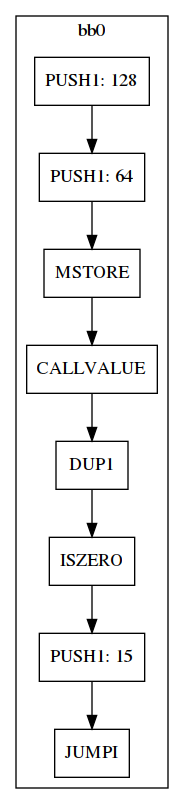
\includegraphics[scale=0.25]{figures/cfg_normalBB0.png}
\end{figure}
}
\only<3-4>{
\begin{figure}
    \centering
    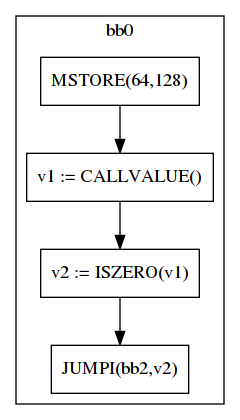
\includegraphics[scale=0.25]{figures/cfg_optimizedBB0.png}
\end{figure}
}
\only<4>{
\begin{figure}
    \centering
    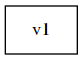
\includegraphics[scale=0.5]{figures/stackBB0.png}
    \caption{Stack state bb0}
\end{figure}
}
\end{columns}
\end{frame}

\begin{frame}{Merging Paths Problem}
\begin{columns}
\column{0.3\textwidth}
\begin{figure}
    \centering
    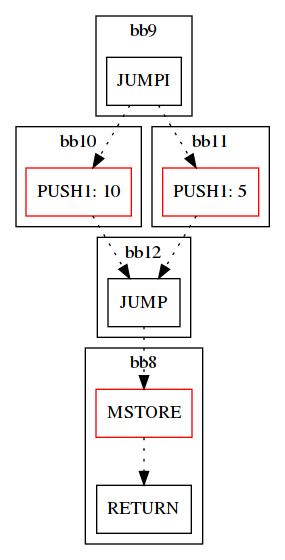
\includegraphics[scale=0.25]{figures/cfg_preAbstract.png}
    \caption{CFG}
\end{figure}
\onslide<2->
\column{0.3\textwidth}
\begin{figure}
    \centering
    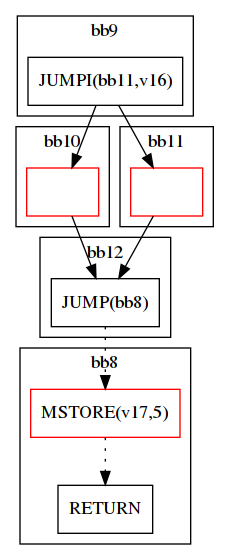
\includegraphics[scale=0.25]{figures/cfg_withEmpty.png}
    \caption{First Idea}
\end{figure}
\onslide<3->
\column{0.3\textwidth}
\begin{figure}
    \centering
    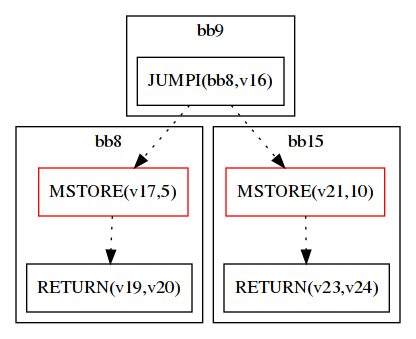
\includegraphics[scale=0.25]{figures/cfg_abstract.png}
    \caption{Second Idea}
\end{figure}
\end{columns}
\end{frame}

\begin{frame}{Stack Abstraction: Second Idea}
\begin{enumerate}
        \item<1-> Replicate the Basic Blocks from the CFG with empty content
        \item \only<1>{Recursive instantiation}\only<2->{Recursive Roll--Out--Instantiation}
            \begin{enumerate}
                \item<2-> \textcolor{red}{Differs the incoming stack to a possibly existing stack?}
                \item<2-> \textcolor{red}{If yes, then create a new BB with the same successors}
                \item<1-> Transform the Operations into Instructions
                \item<1-> Pass the stack to successors
            \end{enumerate}
        \item<2-> \textcolor{red}{Remove Empty and Jump--only Basic Blocks}
    \end{enumerate}
\end{frame}

\begin{frame}{Evaluation: Usefulness of the second Idea}
    \begin{tabu} to \textwidth {| X[c] | X[c] |  X[c] | X[c] | X[c] | }
    \hline
    Bytes in Bytecode & BBs\footnotemark with Operations & Operations & BBs with Instructions & Instructions\\
    \hline
    166 & 13 & 107 & 16 & 39 \\
    \hline
    267 & 16 & 185 & 17 & 54 \\
    \hline
    252 & \textcolor{red}{22} & 179 & \textcolor{red}{32} & 72 \\
    \hline
    313 & 18 & 217 & 19 & 67 \\
    \hline
    \end{tabu}
    \footnotetext[2]{\href{https://www.usenix.org/system/files/conference/usenixsecurity18/sec18-zhou.pdf}{Erays}: Average Smart Contract contains 100 Basic Blocks with an average of 15 Instructions each}
\end{frame}

\begin{frame}{Stack Abstraction Algorithm}
\begin{columns}
\column{0.7\textwidth}
\begin{enumerate}
    \item Replicate the Basic Blocks from the CFG as empty structure
    \item \only<1>{Recursive instantiation}\only<2-3>{\textcolor{red}{Abstract for each bb}}
        \begin{enumerate}
            \item<2-> \textcolor{red}{Retrieve the stack from each predecessor and merge (same variable)}
            \item<1-> Transform the Operations into Instructions
            \item<1-> \textcolor{red}{Store} the state of the stack
        \end{enumerate}
\end{enumerate}
\column{0.3\textwidth}
\onslide<3->
\begin{figure}
    \centering
    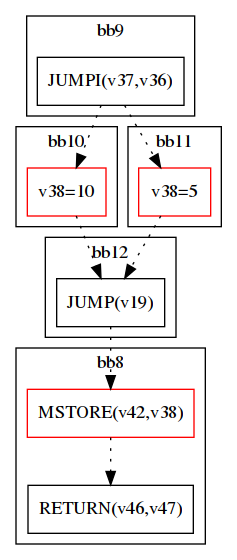
\includegraphics[scale=0.25]{figures/cfg_abstract2.png}
\end{figure}
\end{columns}
\end{frame}

\section{Evaluation}
\begin{frame}{Evaluation Elements}
    \begin{itemize}
        \item<1-> Operators (e.g. $+$,$*$,$\ll$)
        \item<2-> Control Structures
            \begin{itemize}
                \item if-else
                \item loops
                \item return, break, continue
            \end{itemize}
        \item<3-> Datatypes (e.g. int, int8, arrays, struct, mapping)
            \begin{itemize}
                \item fixed length
                \item dynamic length
            \end{itemize}
        \item<4-> Functions (local, global)
    \end{itemize}
\end{frame}

\begin{frame}{Evaluation Items}
    \begin{table}[htb!]
\centering
\begin{tabular}{ | c | c | c | c | c | c | }
\hline
ID & Name & CFG & Optimized & LOC &  Bytes\\
\hline
1 & 1f\_if & yes & yes & 5 & 166\\
2 & 2f & yes & yes & 6 & 267\\
3 & 2f\_if & yes & yes & 8 & 212\\
4 & 2f\_ifif & yes & yes & 15 & 252\\
5 & 2f\_for\_break & yes & \textcolor{red}{no} & 11 & 227\\
6 & 2f\_doWhileIf & yes & \textcolor{red}{no} & 12 & 219\\
7 & 2f\_ifWhile & yes & yes & 11 & 243\\
8 & 1f\_3-level-if & yes & yes & 14 & 234\\
9 & 1f\_string & yes & \textcolor{red}{no} & 3 & 275\\
10 & 1f\_if\_string & yes & \textcolor{red}{no} & 6 & 385\\
11 & 1f\_string\_concat & \textcolor{red}{no} & \textcolor{red}{no} & 8 & 818\\
\ldots & \ldots & \ldots & \ldots & \ldots & \ldots \\
24 & blind\_auction & \textcolor{red}{no} & \textcolor{red}{no} & 52 & 3066\\
\hline
\end{tabular}
\caption{List of test examples. Displays whether the Base CFG and the optimized CFG can process the test correctly. Lines of code (LOC) and the number of Bytes in the Bytecode indicate the size of the test.}
\label{tab:eval}
\end{table}
\end{frame}

\begin{frame}{Other approaches}
Decompiler (Solidity):
    \begin{enumerate}
        \item \href{https://github.com/comaeio/porosity}{Porosity}: Decompiler (Solidity)
        \item \href{https://eveem.org/}{Eveem}: Decompiler (Solidity)
    \end{enumerate}
Security Analysis Frameworks:
    \begin{enumerate}
        \item \href{https://www.usenix.org/system/files/conference/usenixsecurity18/sec18-zhou.pdf}{Erays}: Optimized CFG, Solidity
        \item \href{https://arxiv.org/pdf/1805.07208.pdf}{EthIR} (Oyente): CFG, Rule--based Instructions
        \item \href{https://www.usenix.org/system/files/conference/usenixsecurity18/sec18-krupp.pdf}{TheEther}: CFG, Generates Exploits
        \item \href{https://arxiv.org/pdf/1809.03981.pdf}{Vandal}: Opcode Representation, BB CFG
    \end{enumerate}
\end{frame}

\end{document}
